\uuid{5hoU}
\chapitre{Topologie}
\niveau{L2}
\module{Analyse}
\sousChapitre{Ouvert, fermé, intérieur, adhérence}
\titre{\'Etude d'un domaine de $\R^2$}
\theme{topologie}
\auteur{Maxime NGUYEN}
\datecreate{2023-03-31}
\organisation{AMSCC}
\difficulte{}
\contenu{

Soit $D = \{(x,y) \in \R^2 \, , \, x > 0 \, , \, x+y \leq 0\}$ un domaine de $\R^2$.  
\begin{enumerate}
	\item Proposer une représentation graphique de $D$. 
	\reponse{ 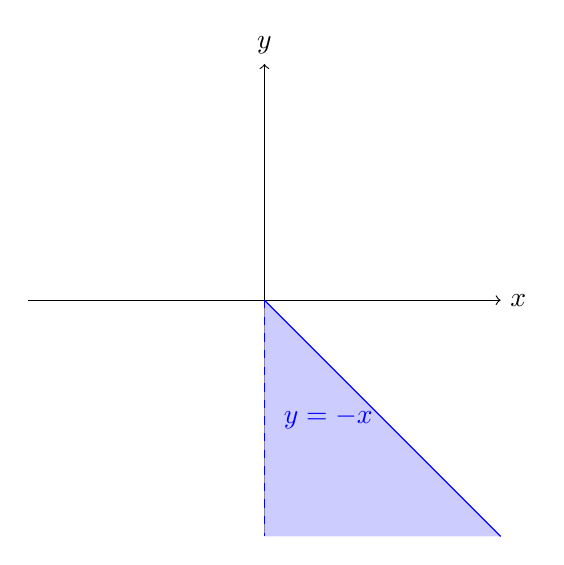
\begin{tikzpicture}[scale=1.5]
			\draw[->] (-2,0) -- (2,0) node[right] {$x$};
			\draw[->] (0,-2) -- (0,2) node[above] {$y$};
			\fill[blue!20,domain=0:2,smooth] (2,-2) -- (0,-2) -- (0,0) -- cycle;
			\draw[blue] (0,0) -- (2,-2) node[midway,left] {$y=-x$};
			\draw[dashed, blue] (0,0) -- (0,-2);
		\end{tikzpicture}
	 }
	\item $D$ est-il ouvert dans $\R^2$ ? justifier rapidement. 
	\reponse{ $D$ n'est pas ouvert dans $\R^2$ car par exemple, le point $(1,-1)$ appartient à $D$ mais aucune boule centrée en ce point de peut être contenue dans $D$. }
	
	\item Vérifier que le point $(0,-1)$ n'appartient pas à $D$. Déterminer une suite de points $(x_n,y_n) \in D$ tels que $(x_n,y_n) \xrightarrow[n \to +\infty]{} (0,-1)$.
	\reponse{ On a  $(0,-1) \notin D$ par définition de $D$, en revanche on peut définir la suite $(x_k,y_k) = (1/k,-1) \in D$ qui converge vers $(0,-1)$. }
	\item $D$ est-il fermé dans $\R^2$ ? justifier rapidement. 
	\reponse{ $D$ n'est pas fermé dans $\R^2$ car par exemple, le point $(2,-2)$ appartient au complémentaire de $D$ et aucune boule centrée en ce point ne peut être contenue dans le complémentaire de $D$. }
	\item \question{ Définir le plus grand ensemble $D'$ inclu dans $D$ de  sorte que $D'$ soit un ouvert de $\R^2$. }
	\reponse{Il suffit d'enlever la droite $x+y=0$ à l'ensemble $D$ pour définir $D' = \{(x,y) \in \R^2 \, , \, x > 0 \, , \, x+y < 0\}$. }
\end{enumerate}}
